%! Tex Program = lualatex
\documentclass[aspectratio=169, 14pt]{beamer}  


\input{./beamer.tex.preamble}

\title{Applied Math 1201B}
\date{Winter 2025}
\author{Kelvin Chan}
\institute{Department of Mathematics\\University of Western Ontario}

\begin{document} 

\begin{frame}
  \maketitle{}
\end{frame}

\section{Course Introduction}

\begin{frame}
  \frametitle{Welcome to ApplMath~1201B! \hfill \parbox{1.25in}{\small Section 001\\MWThF at 8:30}}

  Check the course website (\href{https://owl.uwo.ca}{\texttt{owl.uwo.ca}}) at least once a week.

  \bigskip
  \begin{minipage}{2in}
    \centering
    \qrcode[height=1in]{https://join.iclicker.com/OFXO}
    \bigskip

    \footnotesize\url{join.iclicker.com/OFXO} 

    \bigskip
    Use your @uwo.ca email
  \end{minipage}
  \begin{minipage}{3.5in}
    Join iClicker for in-class activities.

    \bigskip
    Count for \(5\%\) of your final grade. \\Completion marks only. 

    \medskip
    The \hlmain{iClicker Student} app is more stable.
  \end{minipage}
\end{frame}

\begin{frame}
  \frametitle{Welcome to ApplMath~1201B! \hfill \parbox{1.25in}{\small Section 003\\MWThF @ 9:30}}

  Check the course website (\href{https://owl.uwo.ca}{\texttt{owl.uwo.ca}}) at least once a week.

  \bigskip
  \begin{minipage}{2in}
    \centering
    \qrcode[height=1in]{https://join.iclicker.com/SLPE}
    \bigskip

    \footnotesize\url{join.iclicker.com/SLPE} 

    \bigskip
    Use your @uwo.ca email
  \end{minipage}
  \begin{minipage}{3.5in}
    Join iClicker for in-class activities.

    \bigskip
    Count for \(5\%\) of your final grade. \\Completion marks only. 

    \medskip
    The \hlmain{iClicker Student} app is more stable.
  \end{minipage}
\end{frame}

\begin{frame}
  \frametitle{Math and Science}

  \begin{center}
    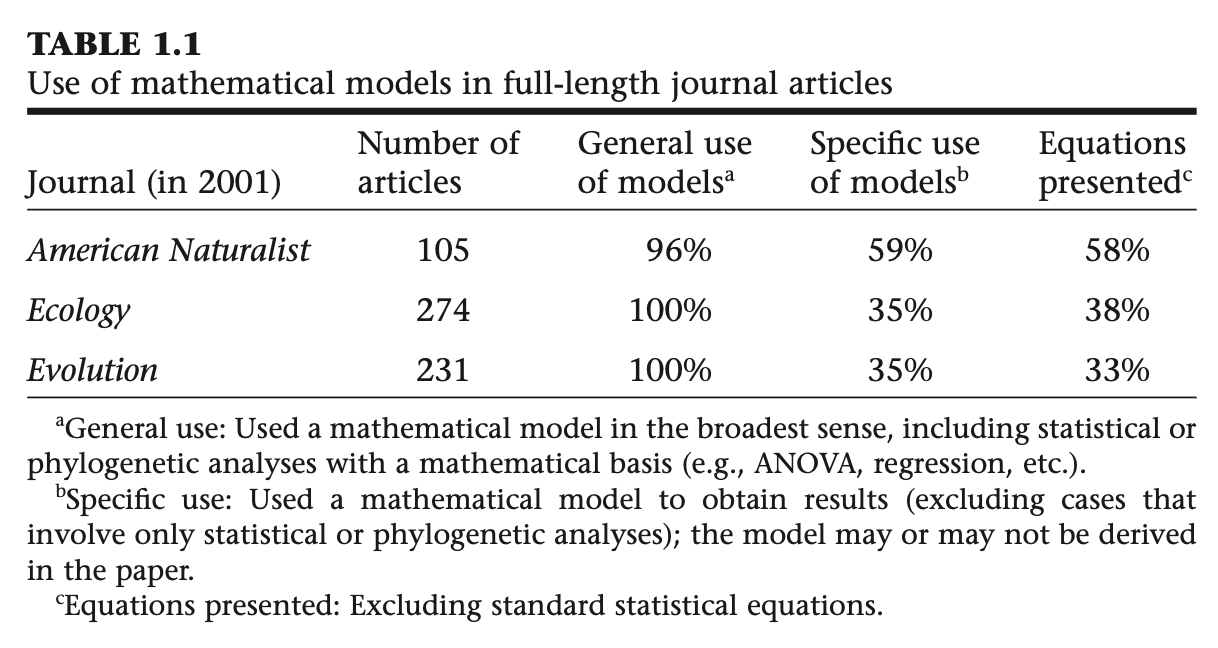
\includegraphics[height=2in]{./standalones/excerpt-otto-day}
  \end{center}

  {\footnotesize An excerpt from \emph{A Biologist's Guide to Mathematical Modelling in Ecology and Evolution} by Sarah P. Otto and Troy Day.}
\end{frame}

\begin{frame}
  \frametitle{Themes in Applied Math 1201}

  The usual math (definitions, ideas, techniques).
  \begin{itemize}
    \item<2-> \hlmain{Discrete-time and continuous-time models}
    \item<3-> \hlmain{Probabilistic model}
    \item<4-> \hlmain{Models with \(2+\) independent variables}
  \end{itemize}

  Use math as a language to build models.

  Use math as a tool to investigate models.

  A tiny bit of scientific computing. How to be a scientist in 2026+
\end{frame}


\section{Scaling Models}
\begin{frame}
  \frametitle{Power rule models and log-log transformations}

  The \hlmain{log-log transformation} of a power rule model \(y = c x^{\alpha}\) is
  \[
    \underbrace{\ln(y)}_{\text{v. axis}} = \overbrace{\alpha}^{\text{slope}} \underbrace{\ln(x)}_{\text{h. axis}} + \overbrace{\ln(c)}^{\text{v. intercept}}.
  \]

  Log-log transformations are ``undoable'' by raising both sides to base \(e\).

  \textbf{A Speedy Notation}. \(y = c x^{\alpha} \longleftrightarrow y \propto x^{\alpha}\). Useful when the constant \(c\) is not important.
\end{frame}

\begin{frame}
  \frametitle{A toucan of truth?}

  \centering

  \includegraphics[page=4, width={2.5in}]{./standalones/plot-birds-of-costa-rica}
  \qquad
  \includegraphics[page=5, width={2.5in}]{./standalones/plot-birds-of-costa-rica}

  How do you evaluate your intern's arguments? 
\end{frame}

\section{Recurrence}
\section{Differential Equations}
\section{Probability}
\section{Random Variables}

\end{document}
